\documentclass[10pt,twocolumn]{article}
\usepackage[margin=1.8cm]{geometry}
\usepackage{graphicx}
\usepackage{amsmath,amssymb}
\usepackage{booktabs}
\usepackage{caption}
\usepackage{hyperref}
\usepackage{xcolor}
\usepackage{subcaption}
\usepackage{enumitem}

\setlist{nosep,leftmargin=*}

\title{FORTE: Force Optimization via Riemannian Trajectory Estimation\\
\large Progress Report}
\author{Ege Doganay \and Furkan B\"{u}y\"{u}ksar{\i}kulak \\
\small Dept.\ of EEE, Bilkent University}
\date{}

\begin{document}
\maketitle

%======================================================================
\section{Introduction}

FORTE (Force Optimization via Riemannian Trajectory Estimation) is a zero-shot framework for contact-rich manipulation. It extends CoRAL~\cite{coral} with: (1)~an online Riemannian Stiffness Estimator on the $\mathcal{S}^3_{++}$ manifold, and (2)~an Energy-Aware MPPI cost with force barriers. All semantic parameters (cost weights, force bands, contact strategies, phase transitions) are generated by GPT-4o from a single scene image and task description.

\subsection{Task: Wall-Assisted Box Lift}

A Panda robot must slide a 16\,cm cube (0.573\,kg) upward along a vertical wall to $h^* = 0.50$\,m using wall friction, without grasping. The box starts on the table surface ($h_0 \approx 0.16$\,m) approximately 3\,cm from the wall. The robot's parallel-jaw gripper cannot grasp the box (max opening $\sim$2\,cm vs.\ 16\,cm box), so it must push from the free face while using wall friction to support the box against gravity.
%======================================================================
\section{Methodology}

\subsection{Pipeline}

\begin{enumerate}
\item \textbf{VLM query.} Scene image $+$ geometry JSON $\to$ GPT-4o $\to$ structured \texttt{PhysicsConfig}: ordered phases with per-phase cost weights $\mathbf{Q}$, force band $[F_{\min},F_{\max}]$, contact strategy, and action prior $\boldsymbol{\mu}$.
\item \textbf{Phase transitions.} \texttt{SemanticManager} evaluates trigger predicates (\texttt{eef\_near\_box}, \texttt{wall\_contact}, etc.) against live metrics and rotates the active cost parameters.
\item \textbf{MPPI planning.} Parallel workers ($N{=}128$, $H{=}12$) evaluate sampled trajectories against the FORTE cost (Eq.~\ref{eq:cost}). 50\% of samples are warm-started from the previous best trajectory.
\item \textbf{Stiffness estimation.} Contact-gated: $\mathbf{K}$ is updated via Riemannian retraction on $\mathrm{SPD}(3)$ only when wall-normal force exceeds 0.5\,N; latched once established.
\end{enumerate}

\subsection{FORTE Cost Function}

Workers evaluate each rollout against Eq.~5 from the proposal~\cite{forte}:
\begin{equation}
J = \underbrace{w_h e_h^2 + w_c e_c^2 + w_p e_p^2}_{\text{Task Tracking}} + \underbrace{\lambda_E\, \boldsymbol{\delta}^\top\!\mathbf{K}\,\boldsymbol{\delta}}_{\text{Energy}} + \underbrace{\rho\,[\bar F]_+^2 + \gamma\,[\underline F]_+^2}_{\text{Force Barriers}}
\label{eq:cost}
\end{equation}
where $e_h{=}\max(0,h^*{-}h)$, $e_c{=}\max(0,g{-}g^*)$ (wall gap), $e_p{=}\|\mathbf{p}_\text{eef}{-}\mathbf{p}_\text{contact}\|$, and the force barriers use MuJoCo sim forces from the rollout. All weights, targets, and force bands originate from the VLM.

%======================================================================
\section{Simulation Environment}

MuJoCo simulation via LIBERO~\cite{libero} with custom extensions.  Key physics parameters (Table~\ref{tab:physics}) were extracted from the simulator after the run to aid failure analysis.

\begin{table}[ht]
\centering\small
\caption{MuJoCo physics parameters.}
\begin{tabular}{@{}lr@{}}
\toprule
Parameter & Value \\
\midrule
Box mass / weight & 0.573\,kg / 5.6\,N \\
Box dimensions & $16 \times 16 \times 16$\,cm \\
Effective contact friction $\mu$ & 1.0 \\
Gripper pad friction & 2.0 \\
Gripper max opening & $\sim$2\,cm \\
OSC position gain $k_p$ & 150 \\
OSC output max & 0.05\,m/step \\
\bottomrule
\end{tabular}
\label{tab:physics}
\end{table}

\begin{figure}[t]
\centering
\begin{subfigure}[b]{0.19\linewidth}
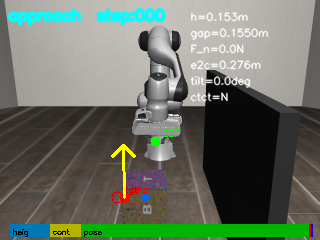
\includegraphics[width=\linewidth]{phase2_figs/frame_000.png}
\caption*{\footnotesize $t{=}0$}
\end{subfigure}
\begin{subfigure}[b]{0.19\linewidth}
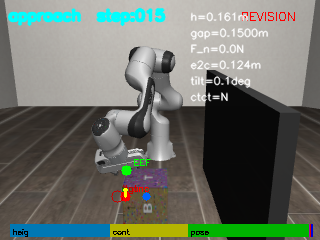
\includegraphics[width=\linewidth]{phase2_figs/frame_015.png}
\caption*{\footnotesize $t{=}15$}
\end{subfigure}
\begin{subfigure}[b]{0.19\linewidth}
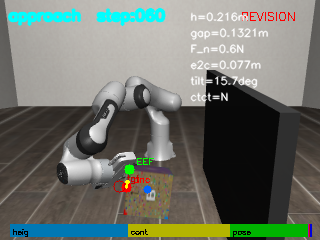
\includegraphics[width=\linewidth]{phase2_figs/frame_060.png}
\caption*{\footnotesize $t{=}60$}
\end{subfigure}
\begin{subfigure}[b]{0.19\linewidth}
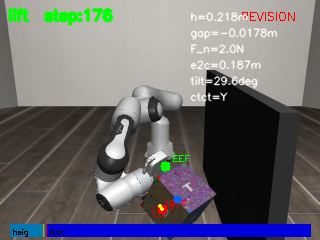
\includegraphics[width=\linewidth]{phase2_figs/frame_176.png}
\caption*{\footnotesize $t{=}176$}
\end{subfigure}
\begin{subfigure}[b]{0.19\linewidth}
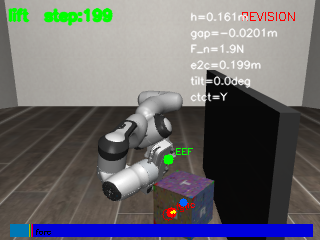
\includegraphics[width=\linewidth]{phase2_figs/frame_199.png}
\caption*{\footnotesize $t{=}199$}
\end{subfigure}
\caption{Rollout snapshots. $t{=}0$: initial. $t{=}15$: approach. $t{=}60$: box at wall. $t{=}176$: peak height. $t{=}199$: settled.}
\label{fig:frames}
\end{figure}

%======================================================================
\section{VLM Zero-Shot Results}

GPT-4o produced a three-phase plan (Table~\ref{tab:phases}) without modification. Phase transitions fired correctly: approach $\to$ push\_to\_wall at step~54, $\to$ lift at step~55. The box reached the wall reliably.

\begin{table}[ht]
\centering\small
\caption{VLM-generated phase plan (zero-shot).}
\begin{tabular}{@{}llcc@{}}
\toprule
Phase & Trigger & $[F_{\min},F_{\max}]$ & $\boldsymbol{\mu}$ \\
\midrule
approach      & \texttt{initial}             & $[0,100]$   & $\mathbf{0}$ \\
push\_to\_wall & \texttt{eef\_near\_box:0.05} & $[0,100]$   & $\mathbf{0}$ \\
lift          & \texttt{wall\_contact}        & $[15,35]$   & $[0,.6,.4,\mathbf{0}]$ \\
\bottomrule
\end{tabular}
\label{tab:phases}
\end{table}

\begin{table}[ht]
\centering\small
\caption{VLM zero-shot run (300 steps, target $h^*{=}0.50$\,m).}
\begin{tabular}{@{}lr@{}}
\toprule
Metric & Value \\
\midrule
Peak height & $\sim$0.22\,m (44\% of target) \\
Sustained lift & 0.06\,m \\
Max normal force & 18.3\,N \\
Max tilt & 28.6$^\circ$ \\
Lateral drift & $+$0.40\,m \\
Success & No \\
\bottomrule
\end{tabular}
\label{tab:summary}
\end{table}

\begin{figure}[ht]
\centering
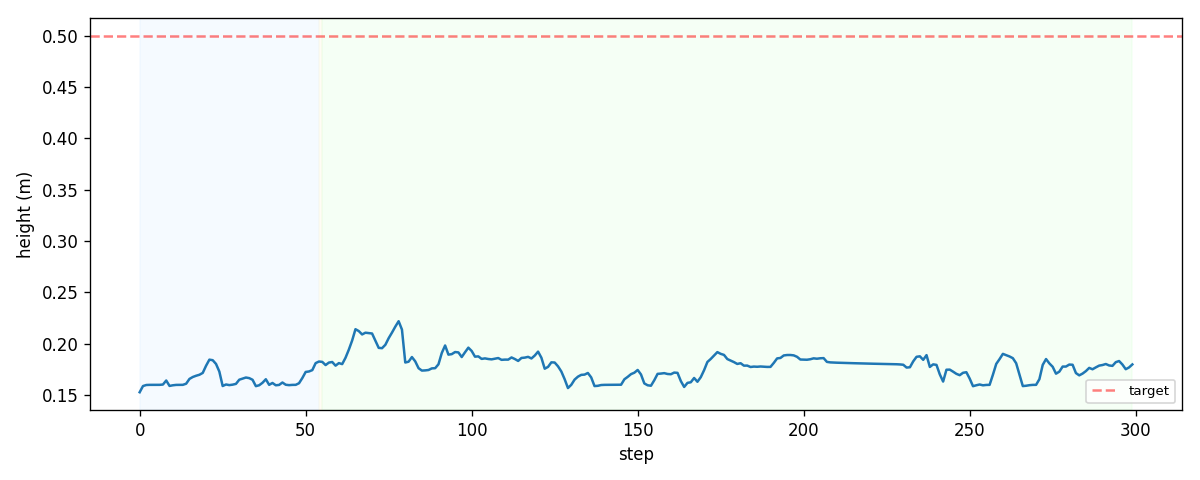
\includegraphics[width=\linewidth]{height_progress.png}
\caption{Box height over time (VLM zero-shot). Sustained 6\,cm lift (0.16\,$\to$\,0.22\,m). The spike near step~110 is a tipping event.}
\label{fig:height}
\end{figure}

\begin{figure}[ht]
\centering
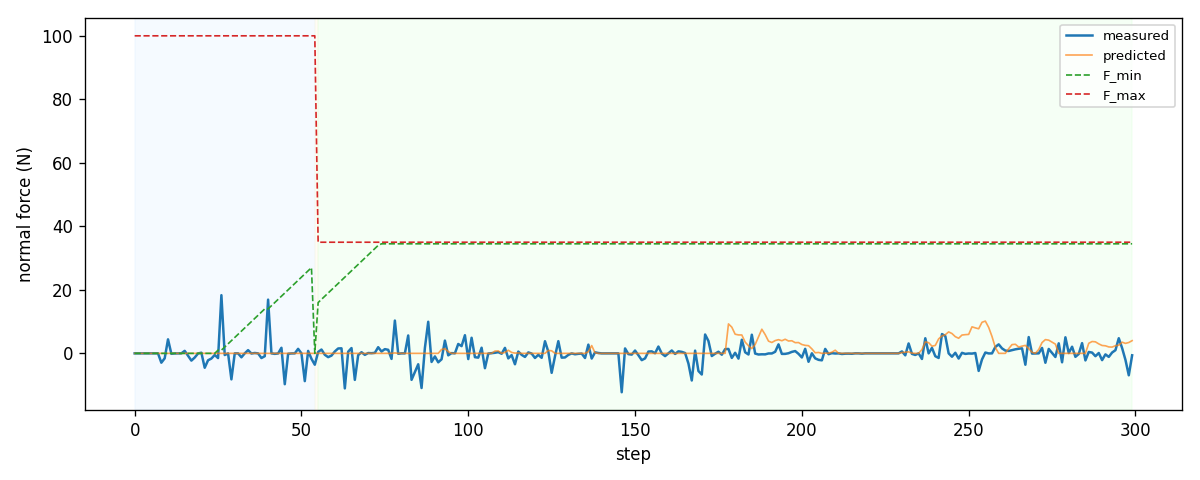
\includegraphics[width=\linewidth]{force_band.png}
\caption{Wall-normal force vs.\ VLM-specified band $[15,35]$\,N. Measured force rarely exceeds 5\,N, far below the friction threshold ($F_n \geq mg/\mu \approx 5.6$\,N).}
\label{fig:force}
\end{figure}

%======================================================================
\section{Failure Analysis}

\subsection{Contact Point Specification}

The primary obstacle is the VLM's ability to specify contact points that produce proper force and torque translation to the object while maintaining an upward wall push. The VLM chose \texttt{contact\_below\_COM} ($-0.5\times$ half-height), placing the target at $z{=}0.013$\,m---below the Panda's reachable workspace. The robot cannot reach this point and instead contacts from above, producing a shallow push angle.

Wall-assisted lift requires push angle $\theta > 45^\circ$ (from horizontal) to overcome friction:
\begin{equation}
F_\text{up} > mg + \mu\, F_n \implies \tan\theta > \mu = 1.0
\end{equation}
At $\theta{=}77^\circ$, only 7.6\,N is needed---within robot capability. But the VLM has no awareness of the robot's kinematic workspace when choosing the contact point.

\subsection{Lateral Drift}

The box drifts $+$40\,cm laterally. The VLM prompt schema did not expose a lateral cost term, so GPT-4o could not penalise drift.

\subsection{Action Saturation}

MPPI worker actions are multiplied $80{\times}8{=}640\times$ before the OSC controller clips to $[-1,1]$. All actions saturate, so MPPI explores only directions, not magnitudes. With both $y$ (wall-push) and $z$ (lift) at max $\to$ $\theta{=}45^\circ$ $\to$ zero net lift at $\mu{=}1.0$.

%======================================================================
\section{Feasibility Study (Hand-Tuned)}

To isolate whether the pipeline \emph{can} succeed given correct parameters, we ran additional experiments with manually tuned defaults (VLM bypassed). These are \textbf{not} zero-shot results; they test infrastructure feasibility.

\begin{table}[ht]
\centering\small
\caption{Hand-tuned iterations (VLM bypassed).}
\begin{tabular}{@{}p{3.5cm}ccc@{}}
\toprule
Change & Peak\,h & Lat. & Tilt \\
\midrule
VLM zero-shot (baseline) & 0.22\,m & 0.40\,m & 65$^\circ$ \\
\midrule
+ lateral cost, OBB gap, dynamic face, tilt penalty & 0.20\,m & 0.17\,m & 25$^\circ$ \\
+ $g^*{=}0$, $F_{\min}{=}1$, $w_h{=}30$ & 0.20\,m & 0.12\,m & 14$^\circ$ \\
+ worker action scaling fix & 0.22\,m & 0.08\,m & 30$^\circ$ \\
\bottomrule
\end{tabular}
\label{tab:handtuned}
\end{table}

The hand-tuned runs fixed lateral drift (0.40\,$\to$\,0.08\,m) and tilt (65$^\circ$\,$\to$\,14$^\circ$) but did not improve peak height beyond 0.22\,m. This confirms the bottleneck is not parameter tuning but the force-angle physics described in Section~5.1.

Infrastructure fixes validated during this study (task-agnostic):
\begin{itemize}
\item OBB-based gap computation under box rotation
\item Dynamic approach face selection (adapts to current orientation)
\item Bounded semantic revision (prevents weight escalation)
\item Lateral stability cost term (now exposed in VLM schema)
\end{itemize}

%======================================================================
\section{Remaining Plan}

\begin{enumerate}
\item \textbf{VLM prompt redesign.} Replace geometric contact parameters with force-direction objectives the planner maps to feasible contacts via the robot's workspace.
\item \textbf{Action scaling fix.} Restore proportional worker scaling to enable force magnitude exploration.
\item \textbf{Multi-task validation.} Test on CoRAL's wall-flip task (proven baseline) then other fundamental tasks to validate the pipeline on a task with known feasibility.
\item \textbf{Novel Tasks} Add more tasks such as deformable objects and force sensitive object cleaning to highlight the performance of Remanian Stifness term. (If time allows add a piano playing task where the robot must distinguish a "pianno" or "forte" expression and strike a mock piano key accordingly :) )
\item \textbf{Ablation.} Riemannian vs.\ diagonal stiffness, with/without contact maintenance.
\end{enumerate}

%======================================================================
\section{Team Contributions}

\begin{itemize}
\item \textbf{Ege Doganay:} Riemannian stiffness estimator, FORTE MPPI pipeline (cost function, phase transitions, semantic revision), VLM prompt engineering, benchmarking pipeline, failure analysis.
\item \textbf{Furkan B\"{u}y\"{u}ksar{\i}kulak:} MuJoCo/LIBERO environment setup, wall-lift task design, benchmarking pipeline.
\end{itemize}

%======================================================================
\section{Supplementary Material}

Three video demonstrations are included with this report that highlights especially the major issue of contact point-sampling/prediction.

%======================================================================
\begin{thebibliography}{9}
\bibitem{coral} B.~Cicek, M.~Er, E.~Doganay, and O.~Oguz, ``CoRAL: Contact-Rich Adaptive LLM-based Control,'' 2025. \url{https://openreview.net/forum?id=qPbDM5LRtE}.
\bibitem{forte} E.~Doganay and F.~B\"{u}y\"{u}ksar{\i}kulak, ``FORTE: Force Optimization via Riemannian Trajectory Estimation,'' Project Proposal, Bilkent University, 2026.
\bibitem{libero} B.~Liu et al., ``LIBERO: Benchmarking Knowledge Transfer for Lifelong Robot Learning,'' in \textit{Proc.\ NeurIPS}, 2023.
\bibitem{foundationpose} B.~Wen et al., ``FoundationPose: Unified 6D Pose Estimation and Tracking of Novel Objects,'' in \textit{Proc.\ CVPR}, 2024.
\bibitem{omnivic} Y.~Zhang et al., ``OmniVIC: A Self-Improving Variable Impedance Controller with Vision-Language In-Context Learning,'' \textit{arXiv:2510.17150}, 2025.
\bibitem{pennec} X.~Pennec, P.~Fillard, and N.~Ayache, ``A Riemannian Framework for Tensor Computing,'' \textit{Int.\ J.\ Computer Vision}, vol.~66, no.~1, 2006.
\end{thebibliography}

\end{document}
